\documentclass[a4paper]{article}
\usepackage[UTF8]{ctex}
\usepackage{geometry}
\usepackage{graphicx}
\usepackage{url}
\usepackage{multirow}
\usepackage{array}
\usepackage{booktabs}
\usepackage{url}
\usepackage{enumitem}
\usepackage{graphicx}
\usepackage{float}
\usepackage{amssymb}
\usepackage{amsmath}
\usepackage{subfig}
\usepackage{longtable}
\usepackage{pifont}
\usepackage{color}

\allowdisplaybreaks

\geometry{a4paper, scale=0.78}

% \begin{figure}[H]
%     \centering
%     \includegraphics[width=.55\textwidth]{E.png}
%     \caption{矩阵与列向量的乘法}
%     \label{fig:my_label_1}
% \end{figure}

% \left\{
% \begin{array}{ll}
%       x+2x+z=2 & \\
%       3x+8y+z=12 & \\
%       4y+z=2
% \end{array}
% \right.

% \begin{enumerate}[itemindent = 1em, itemsep = 0.4pt, parsep=0.5pt, topsep = 0.5pt]

% \end{enumerate}

%\stackrel{a}{\longrightarrow}

%\underbrace{}_{} %下括号

%\tableofcontents %目录,并且目录页不记录页码
% \tableofcontents
% \newpage
% \setcounter{page}{1} %new page
% \clearpage

\title{Hidden Markov Model 02 Evaluation}
\author{Chen Gong}
\date{08 January 2020}

\begin{document}
\maketitle
Evaluation的问题可以被我们描述为:给定一个$\lambda$,如何求得$P(O|\lambda)$。也就是在给定模型$\lambda$的情况下,求某个观测序列出现的概率。

\section{模型求解}
对于$P(O|\lambda)$我们利用概率的基础知识进行化简可以得到:
\begin{equation}
    P(O|\lambda) = \sum_{I}P(O,I|\lambda) = \sum_{I}P(O|I,\lambda)P(I|\lambda)
\end{equation}

其中$\sum_{I}$表示所有可能出现的隐状态序列;$\sum_{I}P(O|I,\lambda)$表示在某个隐状态下,产生某个观测序列的概率;$P(I|\lambda)$表示某个隐状态出现的概率。

那么:
\begin{equation}
    \begin{split}
        P(I|\lambda) = & P(i_1,\cdots,i_T|\lambda) \\
        = & P(i_T|i_1,\cdots,i_{T-1},\lambda)\cdot P(i_1,\cdots,i_{T-1}|\lambda) \\
    \end{split}
\end{equation}

根据Hidden Markov Model两个假设中的,齐次马尔可夫假设,我们可以得到:$P(i_T|i_1,\cdots,i_{T-1},\lambda) = P(i_T|i_{T-1}) = a_{i_{T-1},i_T}$。后面按照一样的思路进行迭代就可以了。那么我们继续对公式(2)进行化简可以得到:
\begin{equation}
    \begin{split}
        P(i_T|i_1,\cdots,i_{T-1},\lambda)\cdot P(i_1,\cdots,i_{T-1}|\lambda) 
        = & P(i_T|i_{T-1}) \cdot P(i_1,\cdots,i_{T-1}|\lambda) \\
        = & a_{i_{T-1},i_T}\cdot a_{i_{T-2},i_{T-1}} \cdots a_{i_1,i_2} \cdot \pi(a_{i_1}) \\
        = & \pi(a_{i_1}) \prod_{t=2}^T a_{i_{t-1},i_t}
    \end{split}
\end{equation}

然后,运用观察独立假设,我们可以知道:
\begin{equation}
    \begin{split}
        P(O|I,\lambda) = & P(o_1,o_2,\cdots,o_T|I,\lambda) \\
        = & \prod_{t=1}^T P(o_t|I,\lambda) \\
        = & \prod_{t=1}^T b_{i_t}(o_t)
    \end{split}
\end{equation}

那么,结合公式(2-5),我们可以得到:
\begin{equation}
\begin{split}
        P(O|\lambda) = & \sum_I  \pi(a_{i_1}) \prod_{t=2}^T a_{i_{t-1},i_t} \prod_{t=1}^T b_{i_t}(o_t) \\
        = & \sum_{i_1}\cdot \sum_{i_2} \cdots \sum_{i_T} \pi(a_{i_1}) \prod_{t=2}^T a_{i_{t-1},i_t} \prod_{t=1}^T b_{i_t}(o_t)
\end{split}
\end{equation}

因为一共有$T$个状态,每个状态有$N$种可能,所以算法复杂度为$\mathcal{O}(N^T)$。既然这样直接求太困难了,我们就需要另外想办法。

\section{Forward Algorithm}
下面,我们首先展示一下Hidden Markov Model的拓扑结构图。
\begin{figure}[H]
    \centering
    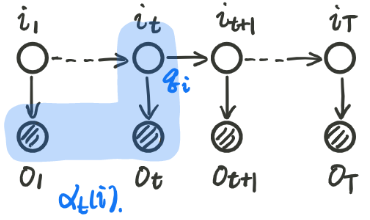
\includegraphics[width=.5\textwidth]{微信图片_20200108102954.png}
    \caption{矩阵与列向量的乘法}
    \label{fig:my_label_1}
\end{figure}

我们记,$\alpha_t(i) = P(o_1,\cdots,o_t,i_t = q_i|\lambda) $,这个公式表示的是在之前所有的观测变量的前提下求出当前时刻的隐变量的概率。那么:
\begin{equation}
    \begin{split}
        P(O|\lambda) = \sum_{i=1}^N P(O, i_t = q_i | \lambda) = \sum_{i=1}^N \alpha_t(i)
    \end{split}
\end{equation}

其中,$\sum_{i=1}^N$表示对所有可能出现的隐状态情形求和,而$\alpha_t(i)$表示对所有可能出现的隐状态情形求和。我们的想法自然就是寻找$\alpha_t(i)$和$\alpha_t(i+1)$之间的关系,这样通过递推,我们就可以得到整个观测序列出现的概率。那么,下面我们来进行推导:
\begin{equation}
    \begin{split}
        \alpha_t(i+1) = & P(o_1,\cdots,o_t,o_{t+1},i_{t+1}=q_j|\lambda) \\
    \end{split}
\end{equation}

因为$\alpha_t(i)$里面有$i_{t}=q_j$,我们就要想办法把$i_{t}$给塞进去,所以:
\begin{equation}
    \begin{split}
        \alpha_t(i+1) 
        = & P(o_1,\cdots,o_t,o_{t+1},i_{t+1}=q_j|\lambda) \\
        = & \sum_{i=1}^N P(o_1,\cdots,o_t,o_{t+1},i_{t}=q_i,i_{t+1}=q_j|\lambda) \\
        = & \sum_{i=1}^N P(o_{t+1}|o_1,\cdots,o_t,i_{t}=q_i,i_{t+1}=q_j,\lambda)
        \cdot P(o_1,\cdots,o_t,i_{t}=q_i,i_{t+1}=q_j|\lambda)
    \end{split}
\end{equation}

又根据观测独立性假设,我们可以很显然的得到$P(o_{t+1}|o_1,\cdots,o_t,i_{t}=q_i,i_{t+1}=q_j,\lambda) = P(o_{t+1}|i_{t+1}=q_j)$。所以:
\begin{equation}
\begin{split}
    \alpha_t(i+1) = & \sum_{i=1}^N P(o_{t+1}|o_1,\cdots,o_t,i_{t} = q_i,i_{t+1}=q_j,\lambda) \cdot P(o_1,\cdots,o_t,i_{t} = q_i,i_{t+1}=q_j|\lambda) \\
    = & \sum_{i=1}^N P(o_{t+1}|i_{t+1}=q_j)\cdot P(o_1,\cdots,o_t,i_{t}=q_i,i_{t+1}=q_j|\lambda)
\end{split}
\end{equation}

看到这个化简后的公式,我们关注一下和$\alpha_t(i)$相比,好像还多了一项$i_{t+1}=q_j$,我们下一步的工作就是消去它。所以:
\begin{equation}
    P(o_1,\cdots,o_t,i_{t}=q_i,i_{t+1}=q_j|\lambda) = P(i_{t+1}=q_j |o_1,\cdots,o_t,i_{t}=q_i,\lambda)\cdot P(o_1,\cdots,o_t,i_{t}=q_i|\lambda) 
\end{equation}

根据齐次马尔可夫性质,我们可以得到$P(i_{t+1}=q_j |o_1,\cdots,o_t,i_{t}=q_i,\lambda) = P(i_{t+1}=q_j = i_{t}=q_i)$。所以根据以上的推导,我们可以得到:
\begin{equation}
    \begin{split}
        \alpha_{t+1}(j) 
        = & \sum_{i=1}^N P(o_{t+1}|i_{t+1}=q_j)\cdot P(i_{t+1}=q_j | i_{t}=q_i) \cdot P(o_1,\cdots,o_t,i_{t}=q_i|\lambda) \\
        = & b_j(o_{t+1})\cdot a_{ij} \cdot \alpha_t(i)
    \end{split}
\end{equation}

经过上述的推导,我们就成功的得到了$\alpha_{t+1}(j)$和$\alpha_t(i)$之间的关系。通过这个递推关系,就可以遍历整个Markov Model了。这个公式是什么意思呢?它可以被我们表达为,所有可能出现的隐变量状态乘以转移到状态$j$的概率,乘以根据隐变量$i_{t+1}$观察到$o_{t+1}$的概率,乘上根据上一个隐状态观察到的观察变量的序列的概率。

我们可以用一个图来进行表示:
\begin{figure}[H]
    \centering
    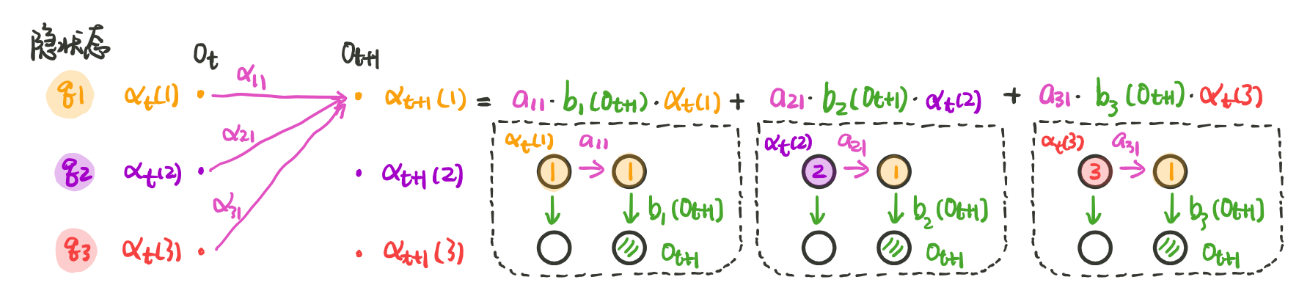
\includegraphics[width=1\textwidth]{微信图片_20200108115145.png}
    \caption{Hidden Markov Model前向传播示意图}
    \label{fig:my_label_1}
\end{figure}

其实读神经网络了解的同学就会发现,这实际上和前向传播神经网络非常的像,实际上就是状态的值乘以权重。也就是对于上一个隐状态的不同取值分别计算概率之后再求和。这样每次计算,有隐状态的状态空间数为$N$,序列的长度为$T$,那么总的时间复杂度为$\mathcal{O}(TN^2)$。

\section{Backward Algorithm}
后向概率的推导实际上比前向概率的理解要难一些,前向算法实际上是一个联合概率,而后向算法则是一个条件概率,所以后向的概率实际上比前向难求很多。
\begin{figure}[H]
    \centering
    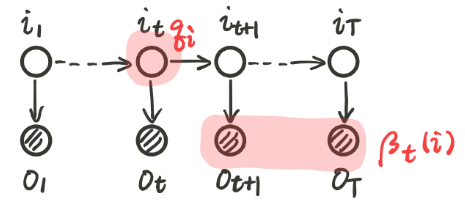
\includegraphics[width=0.5\textwidth]{微信图片_20200108150401.png}
    \caption{Hidden Markov Model后向算法示意图}
    \label{fig:my_label_1}
\end{figure}

我们设$\beta_t(i)= P(o_{t+1},\cdots,o_T|i_t = q_i,\lambda)$,以此类推,$\beta_t(1)= P(o_{2},\cdots,o_T|i_1 = q_i,\lambda)$。我们的目标是计算$P(O|\lambda)$的概率,我们首先来推导一下这个公式:
\begin{equation}
    \begin{split}
        P(O|\lambda) 
        = & P(o_1,o_2,\cdots,o_N|\lambda) \\
        = & \sum_{i=1}^N P(o_1,o_2,\cdots,o_N,i_1=q_i|\lambda) \\
        = & \sum_{i=1}^N P(o_1,o_2,\cdots,o_N|i_1=q_i, \lambda)P(i_1=q_i|\lambda) \\
        = & \sum_{i=1}^N P(o_1| o_2,\cdots,o_N, i_1=q_i, \lambda)\cdot P(o_2,\cdots,o_N, i_1=q_i | \lambda) \cdot \pi_i \\
        = & \sum_{i=1}^N P(o_1| i_1=q_i,\lambda) \cdot \beta_1(i) \cdot \pi_i \\
        = & \sum_{i=1}^N b_i(o_1) \cdot \pi_i \cdot \beta_1(i) \\
    \end{split}
\end{equation}

现在我们已经成功的找到了$P(O|\lambda)$和第一个状态之间的关系。其中,$\pi_i$为某个状态的初始状态的概率,$b_i(o_1)$表示为第$i$个隐变量产生第1个观测变量的概率,$\beta_1(i)$表示为第一个观测状态确定以后生成后面观测状态序列的概率。结构图如下所示:
\begin{figure}[H]
    \centering
    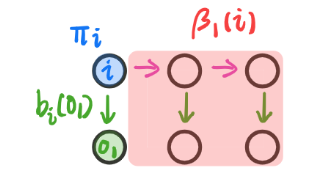
\includegraphics[width=0.4\textwidth]{微信图片_20200108154910.png}
    \caption{$P(O|\lambda)$与第一个状态之间的关系结构图}
    \label{fig:my_label_1}
\end{figure}

那么,我们下一步要通过递推,找到最后一个状态与第一个状态之间的关系。下面做如下的推导:
\begin{equation}
    \begin{split}
        \beta_t(i) 
        = & P(o_{t+1},\cdots,o_T|i_t = q_i)  \\
        = & \sum_{j=1}^N P(o_{t+1},\cdots,o_T, i_{t+1} = q_j|i_t = q_i) \\
        = & \sum_{j=1}^N P(o_{t+1},\cdots,o_T |i_{t+1} = q_j, i_t = q_i)\cdot \underbrace{P(i_{t+1} = q_j|i_t = q_i)}_{a_{ij}} \\
        = & \sum_{j=1}^N P(o_{t+1},\cdots,o_T |i_{t+1} = q_j)\cdot a_{ij} \\
        = & \sum_{j=1}^N P(o_{t+1}|o_{t+2} \cdots,o_T,i_{t+1} = q_j)\cdot \underbrace{P(o_{t+2} \cdots,o_T|i_{t+1})}_{\beta_{t+1}(j)} \cdot a_{ij} \\
        = & \sum_{j=1}^N P(o_{t+1}|i_{t+1} = q_j ) \cdot \beta_{t+1}(j)\cdot a_{ij} \\
        = & \sum_{j=1}^N b_j(o_{t+1}) \cdot \beta_{t+1}(j)\cdot a_{ij}
    \end{split}
\end{equation}

其中第三行到第四行的推导$P(o_{t+1},\cdots,o_T |i_{t+1} = q_j, i_t = q_i) = P(o_{t+1},\cdots,o_T |i_{t+1} = q_j)$使用的马尔可夫链的性质,每一个状态都是后面状态的充分统计量,与之前的状态无关。通过这样的迭代从后往前推,我们就可以得到$\beta_i(1)$的概率,从而推断出$P(O|\lambda)$。整体的推断流程图如下图所示:
\begin{figure}[H]
    \centering
    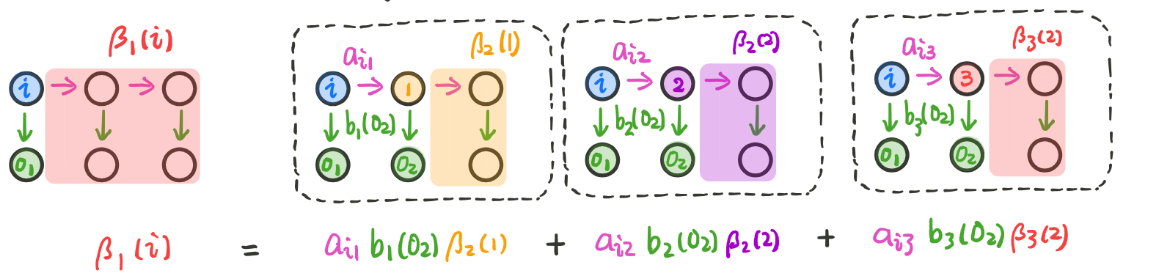
\includegraphics[width=1\textwidth]{微信图片_20200109151358.png}
    \caption{Hidden Markov Model后向算法拓扑结构图}
    \label{fig:my_label_1}
\end{figure}


\end{document}
